
\begin{center}
\textbf{Лабораторная работа №1}
\\
\textbf{Тема:} Работа с системами контроля версий.
\\
Цель:В ходе лабораторной работы необходимо научится работать с системой кантроля версий 
\end{center}

Задание:
\begin{enumerate}

\item Зарегистрироваться на https://github.com/
\item Склонировать репозиторий шаблонов tex https://github.com/egorpugin/tex
\item Подготовить шаблон отчёта для лабораторных работ в LaTeX.
\item Загрузить шаблон в репозиторий tex.
\item Создать новый репозиторий для лабораторных работ на гитхабе.
\item Оформить отчёт и загрузить его в репозиторий для ЛР.
\end{enumerate}

\begin{enumerate}
\item Выполняем каманду git init.
\item Создаем текстовый файл.
\item Создаем репризиторий
\item Загружаем Файл на гит хаб
\end{enumerate}

На данном рисунке изображенл выполнение каманды git init.

\begin{figure}[]% добавляем рисунок.
\centering
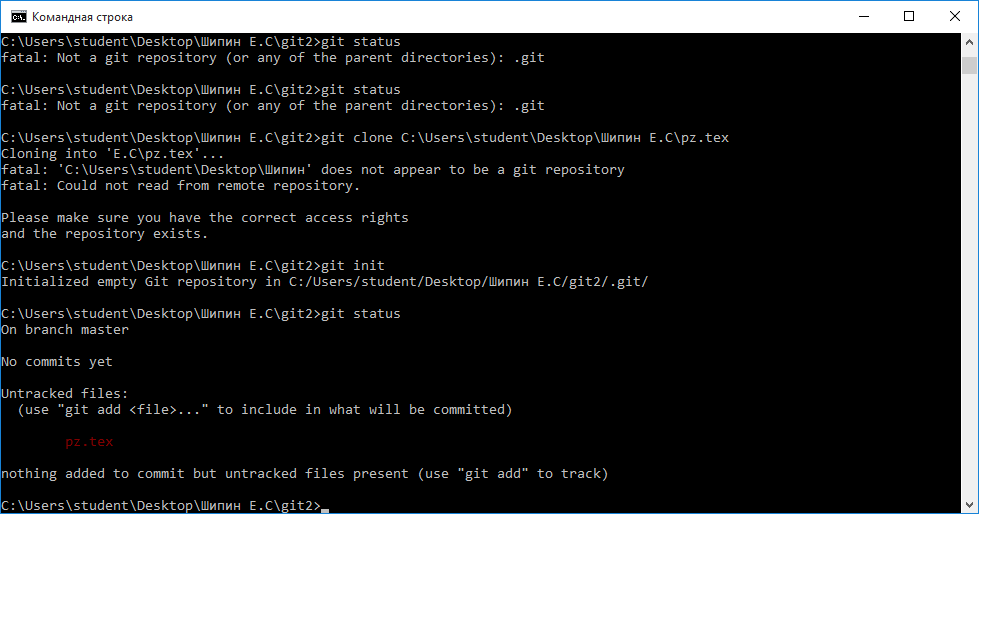
\includegraphics[scale=0.6]{gitin}
\caption{Ваполнение каманды git init}
\label{fig:gitin}
\end{figure}


На данном рисунке изображон созданный репризиторий.

\begin{figure}[]% добавляем рисунок.
\centering
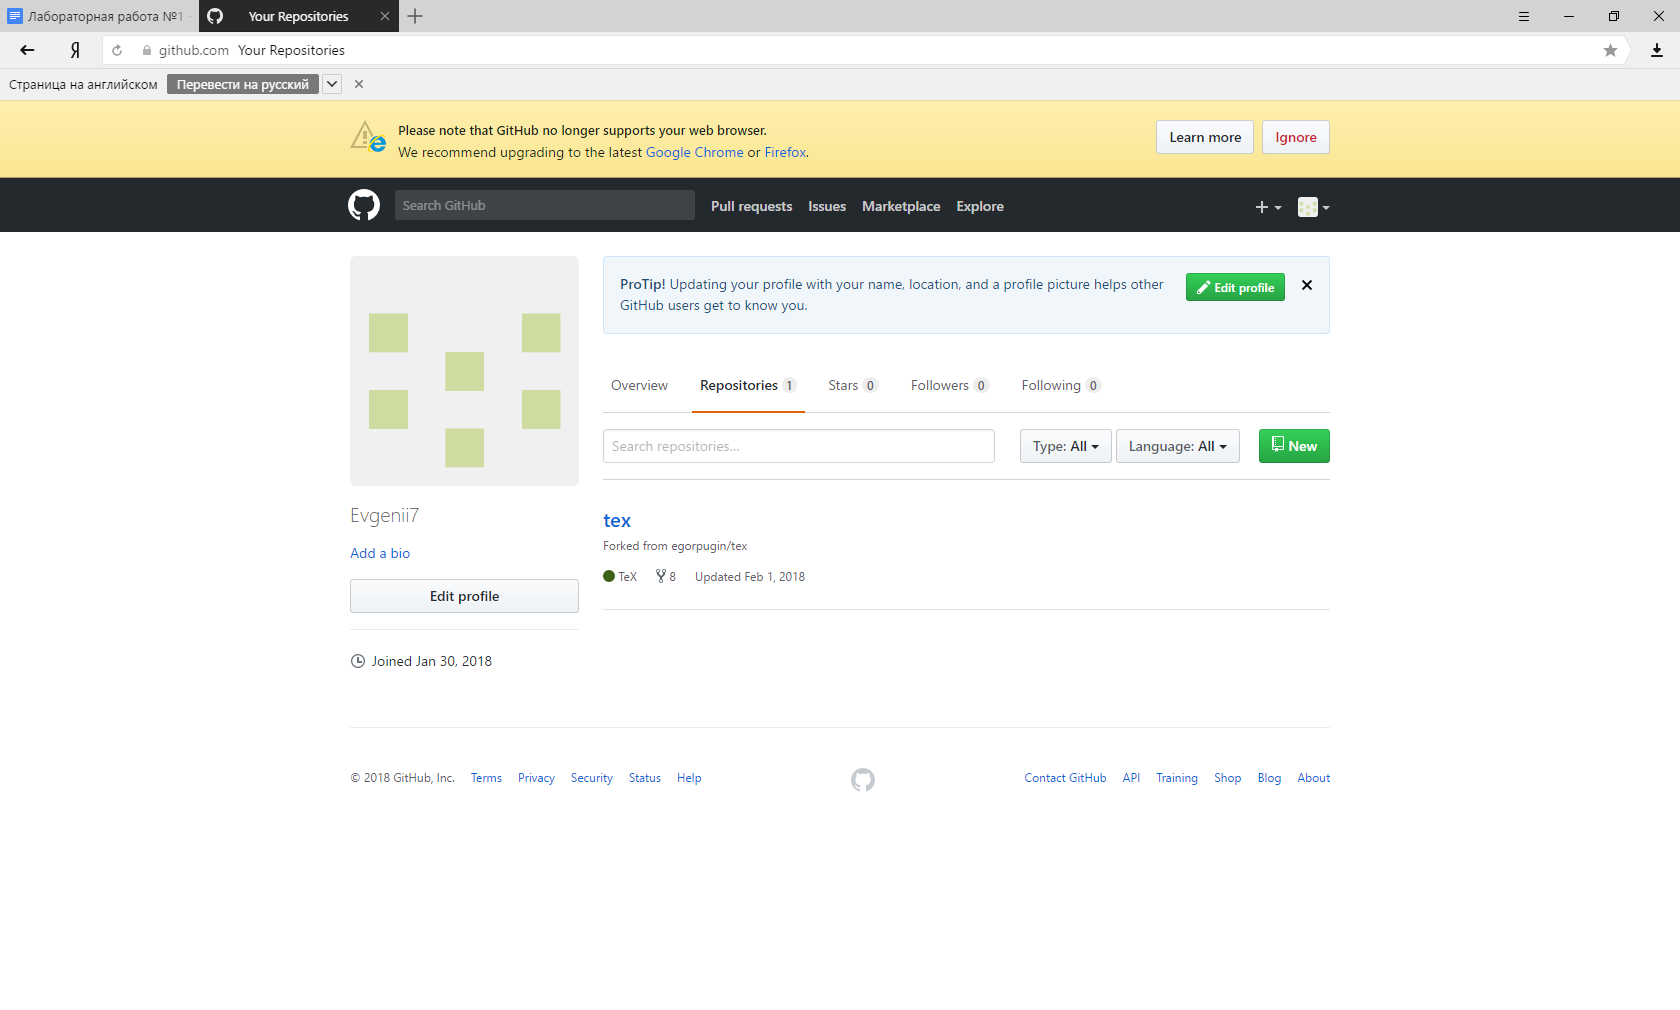
\includegraphics[scale=0.3]{repriz}
\caption{Созданный репризиторий}
\label{fig:repriz}
\end{figure}


\begin{figure}[]% добавляем рисунок.
\centering
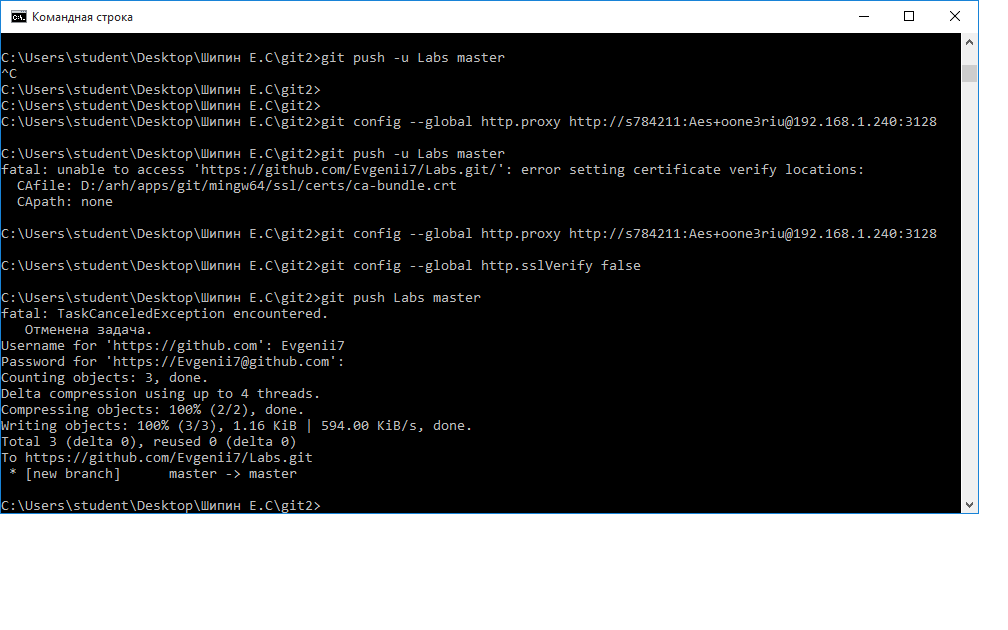
\includegraphics[scale=0.6]{g}
\caption{Добавление файла на гид хаб}
\label{fig:g}
\end{figure}

\newpage
\textbf{Вывод:}
В ходе лаборпторной работы я научился работать с системой контроля версий.




